\documentclass[
10pt,
a4paper,
]{article}
\usepackage{eurosym,natbib,alifeconf}
\usepackage[pdfborder={0 0 0},pdfhighlight=/P]{hyperref}
\usepackage[landscape,twocolumn]{geometry}
\title{The Pop Button}
\author{Kentin$^{1}$ \and Nil$^{2}$ }

\begin{document}
\maketitle
\center{
	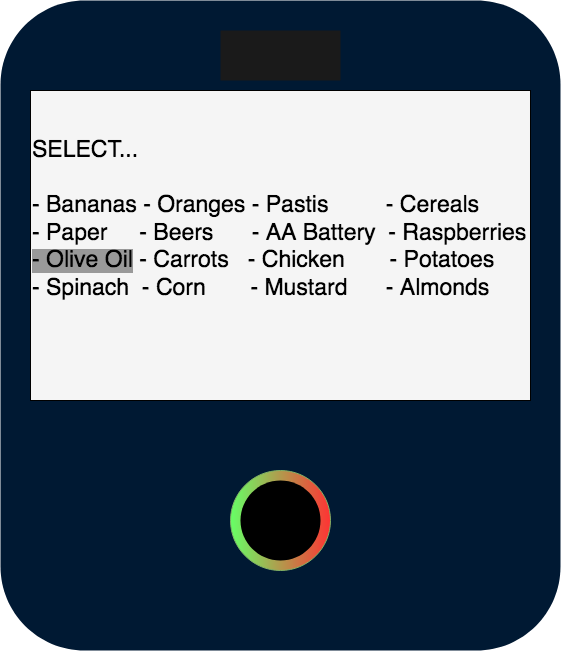
\includegraphics[width=7cm]{pop_button.png}
}

\section{Introduction}
The device consist of a "rotate and push" button, a wi-fi module to communicate with a http server, a screen, a battery holder and of course a PIC32 System on Chip\\
Once turned on the device update his database from the server, load it into the ram and disconnect itself.\\
After 10 seconds the screen goes down and the pic32 goes in sleep mode waiting for the photo-diode or the button to turn it on again.\\
When turned on the wi-fi module try to connect to his base and the screen shows the start of the list, the user can either choose a product he wants to be added to his order list or long push the button to enter the parameters.\\
If the user choose a item this one is added to a temporary stack waiting for the wi-fi to connect, if the connection has not been established the user is warned by a sound and the encoder start to flash red, if everything gone right another sound inform the user that the request had been proceeded  
The parameters menu allows the user to change the contrast of the screen the size of the font and enter the wi-fi password and ssid

\section{Block Diagram}
This is a basic block diagram describing the architecture of the device
\begin{center}
	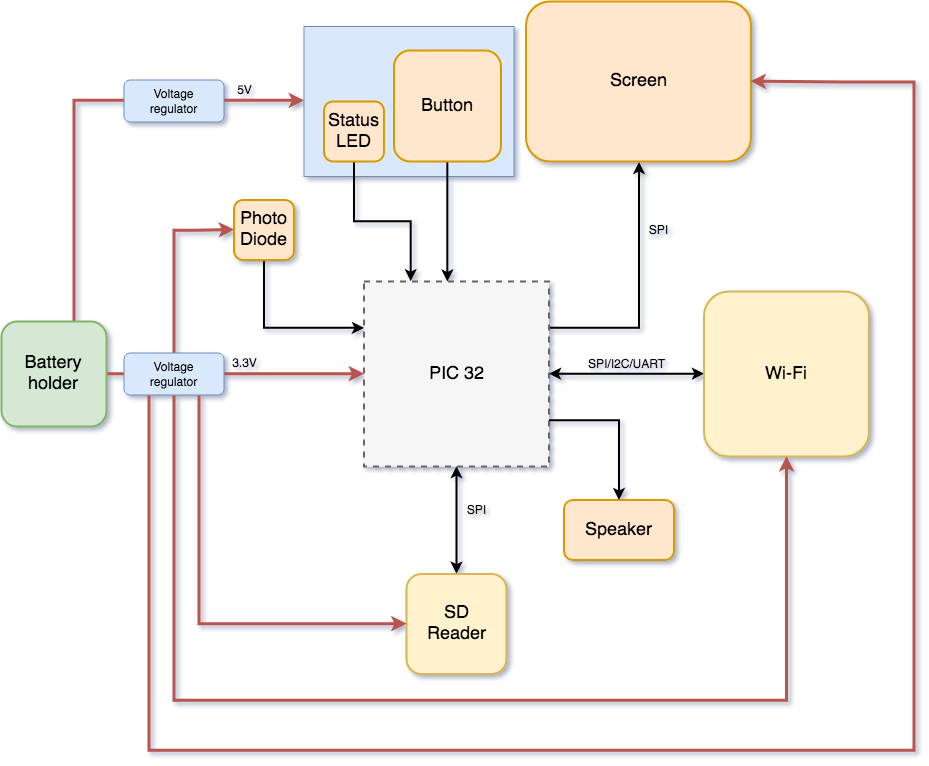
\includegraphics[width=10cm]{block-diagram.png}
\end{center}

\section{Manual}
\subsection{What it does}
The principal purpose of the pop button is to choice in a list what we want to order for the next time you go to the shop or do your weekly/monthly order to you preferred provider
\subsection{Basic use}
\begin{itemize}
	\item You have to activate the switch inside the Pop Button in order to use it, it is placed next to the battery holder and the SD card slot. 
	          
	\item Thanks to his photo-diode turning on the device can be accomplished by passing your hand in front of it or directly pushing the button once.
	          
	\item Once the device is on you can see some items on the screen, you can easily change the current one by turning the rotary button, once you found the object of your desire you can push the button and it will light up green or red depending on the possibility to order your choice.
	          
	\item The list is composed on the server and sent to the device thanks to his wi-fi module, it is stored in the SD card so the list can be long 
	          
	\item In order to connect the device to your network you can either use the SD card to change the configuration file with your computer or long push the button ,enter the appropriated menu and enter the password using the button
	          
\end{itemize}

\section{UART}
UART stand for "Universal Asynchronous Receiver Transmitter" it is a little circuit in a micro-controller which transmit and receive serial data.
As it doesn't use clock it needs to work on a fixed frequency known as the baud rate, the baud rate is explained as bits per second (bps) and both peripherals needs to work on the same one in order to communicate.
UART transmitted data are packets which consist of 1 start bit, 5 to 9 data bits, an optional parity bit, and 1 or 2 stop bits.
\begin{center}
	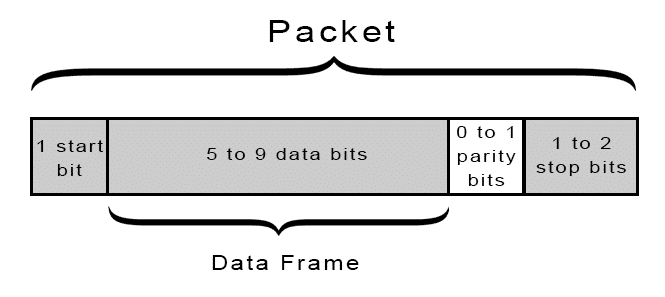
\includegraphics[width=9cm]{UART_packet.png}
\end{center}

\section{SPI}
SPI stand for "Serial Peripheral Interface" it is a communication protocol synchronous and full-duplex which means that it uses a clock and it can receive and send at the same time\\
\subsection{}
This protocol need 3 pins in order to work and uses one pin more for each slaves to select them 
\begin{itemize}
	\item SCLK $\Rightarrow$ Serial Clock\\
	      (SCK, SCL)
	\item MOSI $\Rightarrow$ Master Output, Slave Input\\
	      (SDI, DI, SI)
	\item MISO $\Rightarrow$ Master Input, Slave Output\\
	      (SDO, SDA, DO, SO)
	\item SS $\Rightarrow$ Slave Select\\
	      (nCS, CS, nSS, STE, CSN)
\end{itemize}
There is 4 modes available to use the clock depending on the peripherals properties\\
\begin{table}[!hbt]
	\begin{center}
		\begin{tabular}{|c|c|c|}\hline
			SPI mode & CPOL & CPHA \\\hline\hline
			0        & 0    & 0    \\\hline
			1        & 0    & 1    \\\hline
			2        & 1    & 0    \\\hline
			3        & 1    & 1    \\\hline
		\end{tabular}
	\end{center}
	\caption{CPOL = Clock Polarity CPHA = Clock Phase}
\end{table}

The master start by pulling down the Slave Select and starting the clock, then it send a Read/Write bit, a multiple/single bit an adress it wants to access. Finnaly it reads or write the actual data


\section{\texorpdfstring{i$^{2}$C}{}}
I$^2$C or IIC stands for Inter-Integrated Circuit, it is a protocol which is synchronous, half-duplex, multi-master and multi-slave. It can adress between 127 and 1024 devices but is slower than spi
\subsection{}
This protocol only needs 2 pins
\begin{itemize}
	\item SCL $\Rightarrow$ Serial Clock Line\\
	\item SDA $\Rightarrow$ Serial Data Line
\end{itemize}
\subsection{timeline}
First the master send a start bit by pulling down the SDA right before the clock, then send the device address (7 or 10 bits), a Read/Write bit and wait for the acknowledgment of the slave. Then send the real data which can be the data adress of the device wait for acknowledgment and start again until the stop signal by pulling up the SDA right after the clock. 
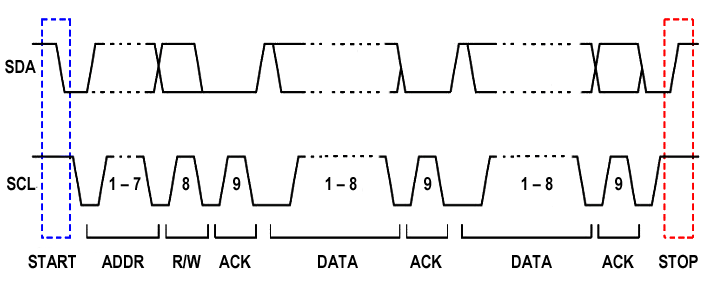
\includegraphics[width=10cm]{i2c.png}


\vskip2.5cm

\begin{center}
	\begin{@twocolumnfalse}
		\begin{table}[!hbt]
			\center{
				\begin{tabular}{|c|c|c|c|c|c|}\hline
					component & reference & price(\euro) & consumption & Frequency & Datasheets \\ \hline\hline
					
					SoC &
					\href{http://fr.farnell.com/microchip/pic32mx174f256b-i-so/mcu-32-bits-pic32mx-72mhz-soic/dp/2775021?st=PIC32MX174F256B}
					{PIC32MX174F256B-I/SO} & 3.48 & $\sim$ 200mA  @ 3.3V = 660mW &
					72Mhz &
					\href{http://www.farnell.com/datasheets/2244305.pdf}{
\includegraphics[height=1em]{pdf.png}}
					\href{http://ww1.microchip.com/downloads/en/DeviceDoc/80000739A.pdf}{
\includegraphics[height=1em]{pdf.png}}\\
					
					Wi-Fi &
					\href{http://fr.farnell.com/microchip/atwinc1500-mr210pb1952/mod-iot-smartconnect-2-472ghz/dp/2759346?st=atwin}
					{ATWINC1500}  & 6.61 & 70mA / 172mA @ 3.3V = 564mW &
					26Mhz &
					\href{http://www.farnell.com/datasheets/2286658.pdf}{
\includegraphics[height=1em]{pdf.png}}\\
					
					Screen &
					\href{http://fr.farnell.com/midas/mccog128064b12w-fptlw/afficheur-lcd-graphique-128x64/dp/2664759}
					{MCCOG128064B12W} & 8.69 & 40mA @ 3.3V = 132mW &
					64hz &
					\href{http://www.farnell.com/datasheets/2151564.pdf}{
\includegraphics[height=1em]{pdf.png}}\\
					
					Rotary Encoder &
					\href{http://fr.farnell.com/bourns/pel12d-2226f-s3024/rotary-encoder-incremental-24/dp/1857558?st=rotary\%20encoder}
					{PEL12D-2226F-S3024} & 1.88 & 10mA @ 5V = 50mW & 
					- &
					\href{http://www.farnell.com/datasheets/1923820.pdf}{
\includegraphics[height=1em]{pdf.png}}\\
					
					Photo-Diode &
					\href{http://fr.farnell.com/optek-technology/opb732/capteur-reflectif-pcb/dp/1226877}
					{OPB732} & 3.2 & 50mA @ 3.3V = 165mW &
					- &
					\href{http://www.farnell.com/datasheets/2331536.pdf}{
\includegraphics[height=1em]{pdf.png}}\\
					    
					Buzzer &
					\href{http://fr.farnell.com/tdk/ps1240p02ct3/buzze-piezoelectronique-3v-4khz/dp/2803350}
					{KPEG242} & 0.591 & 7mA @ 12V = 0.084 &
					- &
					\href{http://fr.farnell.com/kingstate/kpeg242/piezo-buzzer-pin-type/dp/1502726}{
\includegraphics[height=1em]{pdf.png}}\\
					    
					Voltage Regulator 3.3V &
					\href{http://fr.farnell.com/texas-instruments/ua78m33cdcy/regul-de-tension-2vdo-0-5a-3-3v/dp/2296031?st=voltage\%20regulator}
					{UA78M33CDCY} &  0,461 & ? &
					- &
					\href{http://www.ti.com/lit/ds/symlink/ua78m.pdf}{
\includegraphics[height=1em]{pdf.png}}\\
					    
					Voltage Regulator 5V &
					\href{http://fr.farnell.com/microchip/mic5219-5-0ym5-tr/ldo-0-5vdo-0-5a-5v-1-5sot23/dp/2510257}
					{MIC5219-5.0YM5-TR} & 0,816  & ? &
					- &
					\href{http://www.farnell.com/datasheets/683599.pdf}{
\includegraphics[height=1em]{pdf.png}}\\
					    
					\hline
					total && 25.728 & 377mA / 479mA & \\
					\hline
				\end{tabular}
			}
			\caption{basic specifications}
		\end{table}
	\end{@twocolumnfalse}
\end{center}


\footnotesize
{
	\mbox{}\\
	$^1$\href{https://profile.intra.42.fr/users/qdurot}{qdurot} \\
	$^2$\href{https://profile.intra.42.fr/users/nburcion}{nburcion}
}

\end{document}